% The positions of a draw get distinct 64-bit blocks: a draw without replacement
% from an urn. Throwing bits away gives every value many balls, which makes
% drawing without replacement almost the same as drawing with replacement.
% Build: see figures/README.md
\documentclass[tikz, border = 6pt]{standalone}
\usepackage[T1]{fontenc}
\usepackage{lmodern}
\usepackage{amsmath}
\usetikzlibrary{calc, arrows.meta, positioning}

\definecolor{c1}{HTML}{2A7AB0}
\definecolor{c2}{HTML}{E08A2C}
\definecolor{c3}{HTML}{5B8C5A}
\definecolor{c4}{HTML}{B5487A}
\definecolor{c5}{HTML}{7A5BB0}
\definecolor{c6}{HTML}{C9B13A}
\definecolor{c7}{HTML}{3AA6A6}
\definecolor{c8}{HTML}{8A6A4A}

\tikzset{
  >={Stealth[length = 2mm]},
  ball/.style = {circle, draw = black!60, line width = 0.3pt,
    minimum size = 3.2mm, inner sep = 0pt},
  gone/.style = {circle, draw = black!60, densely dashed, line width = 0.4pt,
    minimum size = 3.2mm, inner sep = 0pt},
  title/.style = {font = \bfseries\small, align = center},
  note/.style = {font = \footnotesize, align = center}
}

% \urn{x}{y}{rows}{colour list}{index of the ball drawn}: balls in rows of 8,
% the drawn one is left as a dashed outline and shown above the urn.
\newcommand{\urn}[5]{%
  \begin{scope}[shift = {(#1, #2)}]
    \draw[line width = 0.9pt, black!70, rounded corners = 4pt]
      (-0.25, 0.45 * #3 + 0.15) -- (-0.25, 0) -- (3.15, 0) -- (3.15, 0.45 * #3 + 0.15);
    \foreach \col [count = \k from 0] in {#4} {
      \pgfmathtruncatemacro{\r}{div(\k, 8)}
      \pgfmathtruncatemacro{\c}{mod(\k, 8)}
      \ifnum\k=#5
        \node[gone] at (\c * 0.41, 0.25 + \r * 0.42) {};
        \node[ball, fill = \col] (drawn) at (1.45, 0.45 * #3 + 0.9) {};
        \draw[->, black!60] (\c * 0.41, 0.25 + \r * 0.42 + 0.2) to[bend left = 20] (drawn.west);
      \else
        \node[ball, fill = \col] at (\c * 0.41, 0.25 + \r * 0.42) {};
      \fi
    }
  \end{scope}%
}

\begin{document}
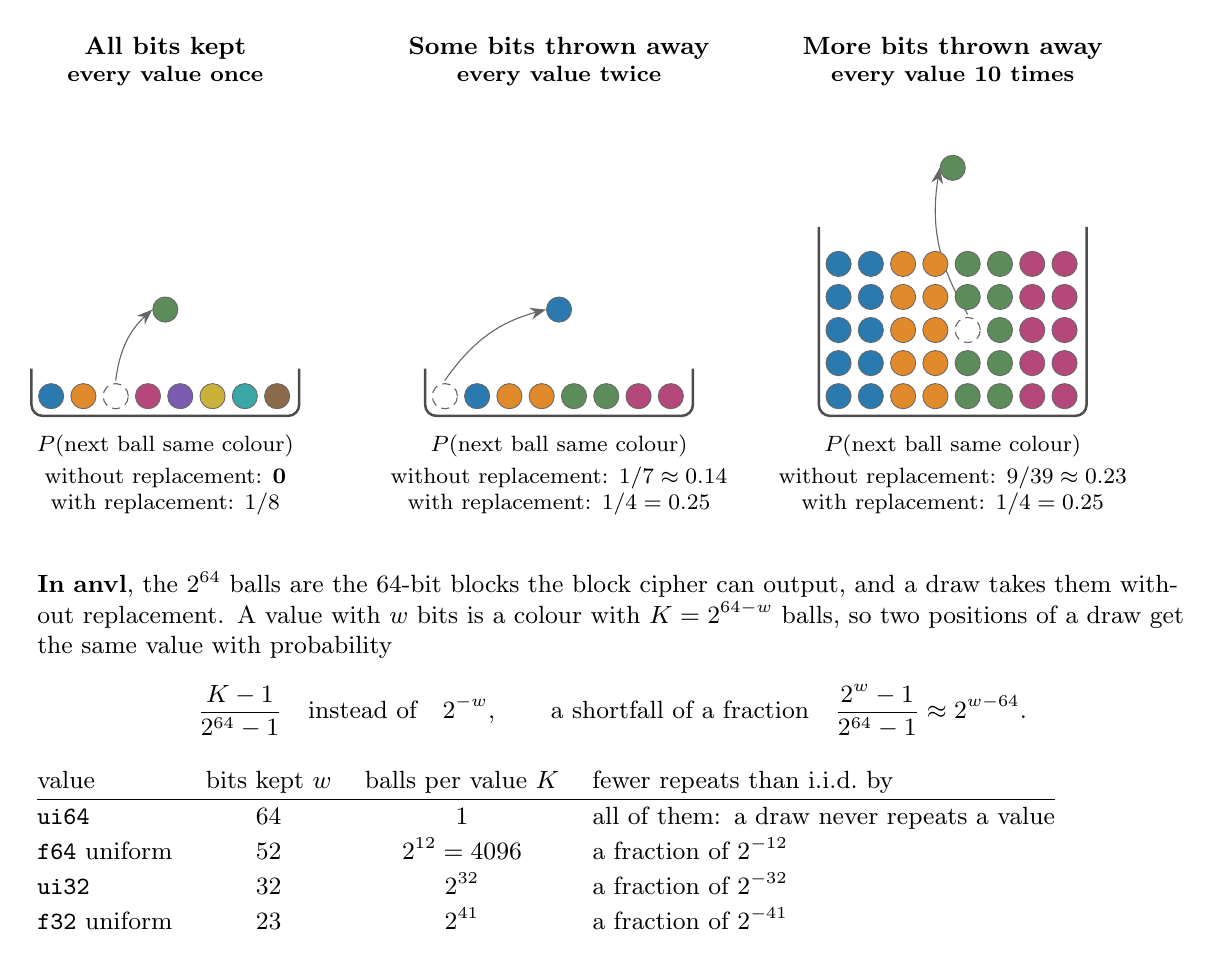
\begin{tikzpicture}[font = \small]

  % ---- (a) keep all 64 bits ---------------------------------------------
  \node[title] at (1.45, 4.5) {All bits kept\\[-1pt]\footnotesize every value once};
  \urn{0}{0}{1}{c1, c2, c3, c4, c5, c6, c7, c8}{2}
  \node[note] at (1.45, -0.75)
    {$P(\text{next ball same colour})$\\[2pt]
     without replacement: $\mathbf{0}$\\
     with replacement: $1/8$};

  % ---- (b) a few balls per colour ---------------------------------------
  \node[title] at (6.45, 4.5) {Some bits thrown away\\[-1pt]\footnotesize every value twice};
  \urn{5}{0}{1}{c1, c1, c2, c2, c3, c3, c4, c4}{0}
  \node[note] at (6.45, -0.75)
    {$P(\text{next ball same colour})$\\[2pt]
     without replacement: $1/7 \approx 0.14$\\
     with replacement: $1/4 = 0.25$};

  % ---- (c) many balls per colour ----------------------------------------
  \node[title] at (11.45, 4.5) {More bits thrown away\\[-1pt]\footnotesize every value 10 times};
  \urn{10}{0}{5}{%
    c1, c1, c2, c2, c3, c3, c4, c4,
    c1, c1, c2, c2, c3, c3, c4, c4,
    c1, c1, c2, c2, c3, c3, c4, c4,
    c1, c1, c2, c2, c3, c3, c4, c4,
    c1, c1, c2, c2, c3, c3, c4, c4}{20}
  \node[note] at (11.45, -0.75)
    {$P(\text{next ball same colour})$\\[2pt]
     without replacement: $9/39 \approx 0.23$\\
     with replacement: $1/4 = 0.25$};

  % ---- in anvl ----------------------------------------------------------
  \node[font = \small, align = left, anchor = north west, text width = 14.6cm]
    at (-0.3, -1.85) {%
    \textbf{In anvl}, the $2^{64}$ balls are the 64-bit blocks the block cipher can output, and a draw
    takes them without replacement.
    A value with $w$ bits is a colour with $K = 2^{64 - w}$ balls, so two positions
    of a draw get the same value with probability
    \[
      \frac{K - 1}{2^{64} - 1} \quad\text{instead of}\quad 2^{-w},
      \qquad\text{a shortfall of a fraction}\quad
      \frac{2^w - 1}{2^{64} - 1} \approx 2^{w - 64}.
    \]
    \renewcommand{\arraystretch}{1.15}%
    \begin{tabular}{@{}lccl@{}}
      value & bits kept $w$ & balls per value $K$ & fewer repeats than i.i.d.\ by \\ \hline
      \texttt{ui64}   & 64 & 1         & all of them: a draw never repeats a value \\
      \texttt{f64} uniform & 52 & $2^{12} = 4096$ & a fraction of $2^{-12}$ \\
      \texttt{ui32}   & 32 & $2^{32}$  & a fraction of $2^{-32}$ \\
      \texttt{f32} uniform & 23 & $2^{41}$  & a fraction of $2^{-41}$ \\
    \end{tabular}};

\end{tikzpicture}
\end{document}
